\chapter{Experiments and Results}
\label{chapter:chapter05}

This chapter presents the core experiments of the research. The main purpose of it was to do a benchmark, as a starting point for the comparison between SOAs and MOAs. The basis for the experimentation layout was based on the experimental framework proposed by H. Ishibuchi, Y. Nojima and T. Doi~\cite{Ishibuchi_single_vs_multiobjective}. \\

The chapter is divided into four different sections, described below:

\begin{itemize}
    \item \textbf{Experiments setup} consists of a set of experiments to determine a reference front to use it for comparison against SOAs and MOAs.
    \item \textbf{First phase} consists of the run of the algorithms without any adjustment using the parameters found in the experimental setup for all the algorithms. This also includes an analysis of the stability of some of the resulting groups.
    \item \textbf{Second phase} takes into account the results of the first phase of experiments and feedback made for its results. It discusses one of the main issues made by the feedback which remarks on whether or not the comparison between SOA and MOA was fair.
    \item \textbf{Third phase} is the result of a discussion about the tuning of parameters. Using only the best algorithms from phase one, chosen by their performance using the parameters from the Experimental setup. 
\end{itemize}

\section{Experiments Setup}

The next section discusses a set of experiments that took place before the core experiments could be made. The first subsection shows the experiment made to search for a reference front for the performance comparison. The next subsection shows an experiment for obtaining the base parameters that would be used to have a fair comparison between the algorithms. The last subsection discusses some of the specific details about each of the individual algorithm implementations.

\subsection{Searching for a Reference Pareto Front}

The IGD+ metric requires to have a defined reference front to perform a proper comparison. To this end, the NSGA-II algorithm was used with a population of 20 individuals for 1000 generations, across 200 independent runs. The best front was chosen considering their HV for each of the problem sizes.\\

After the experiment, the results of each run were compared with each other, and the ones with the lowest HV were chosen. These results are shown in Figures~\ref{fig:reference_front_20}~to~\ref{fig:reference_front_2000} for each respective problem. An important observation is that, in n=20 and n=200, some of the individuals had the same value for each of their objective functions. This observation is important because it is an indication that a global minimum for these problems may exist and could be found using an SOA.\\

\begin{figure}[H]
    \centering
    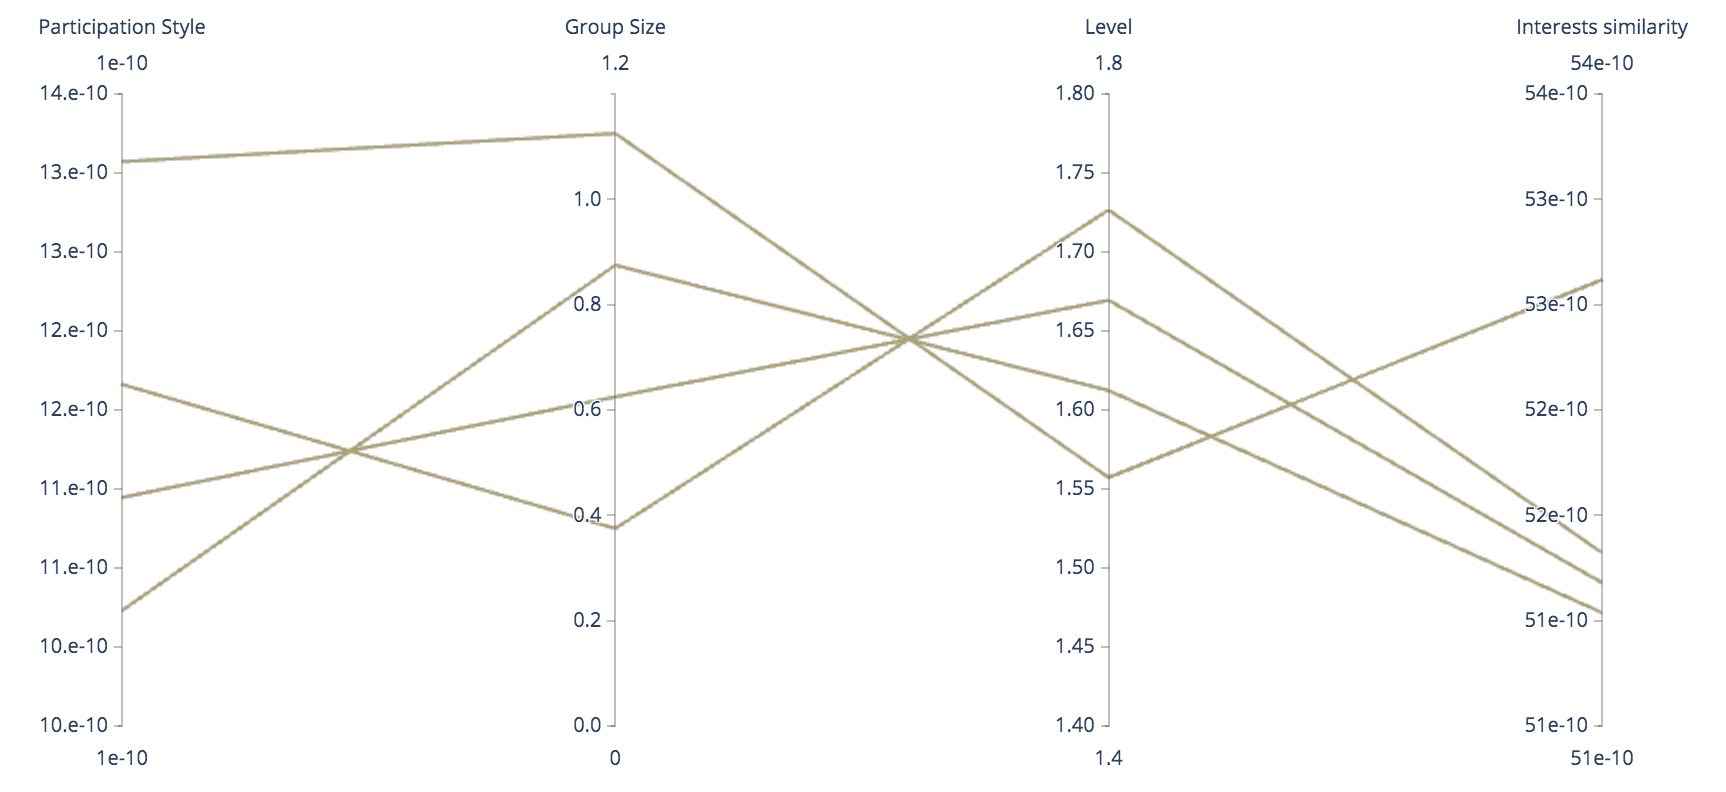
\includegraphics[width=\textwidth]{images/parallel_ref_20.png}
    \caption{Reference front for the $n=20$ problem.}
    \label{fig:reference_front_20}
\end{figure}

\begin{figure}[H]
    \centering
    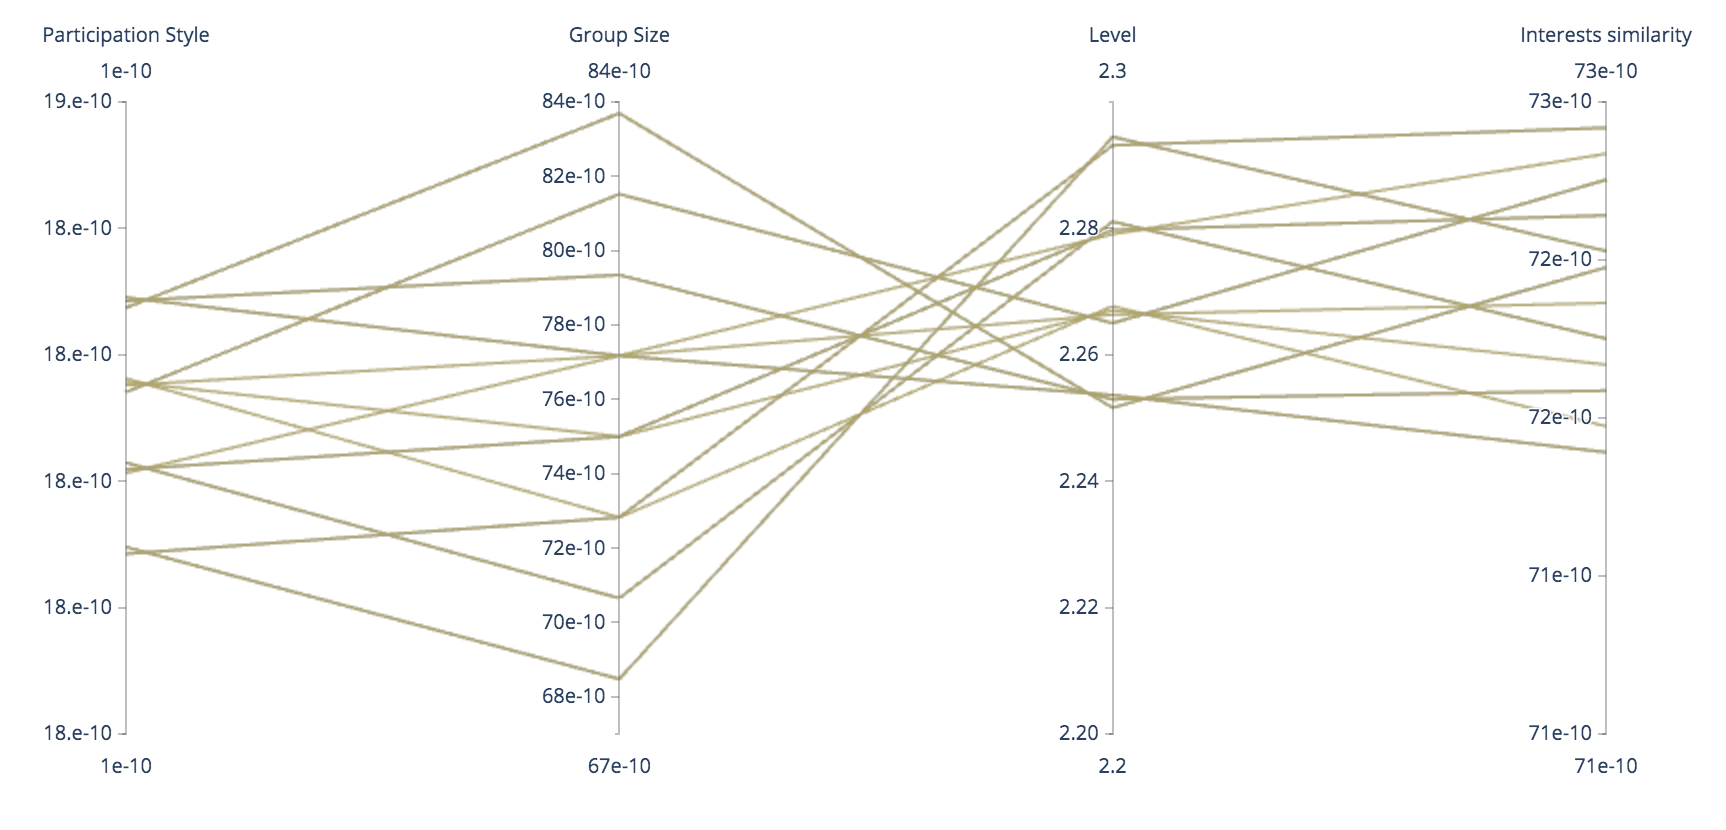
\includegraphics[width=\textwidth]{images/parallel_ref_200.png}
    \caption{Reference front for the $n=200$ problem. }
    \label{fig:reference_front_200}
\end{figure}

\begin{figure}[H]
    \centering
    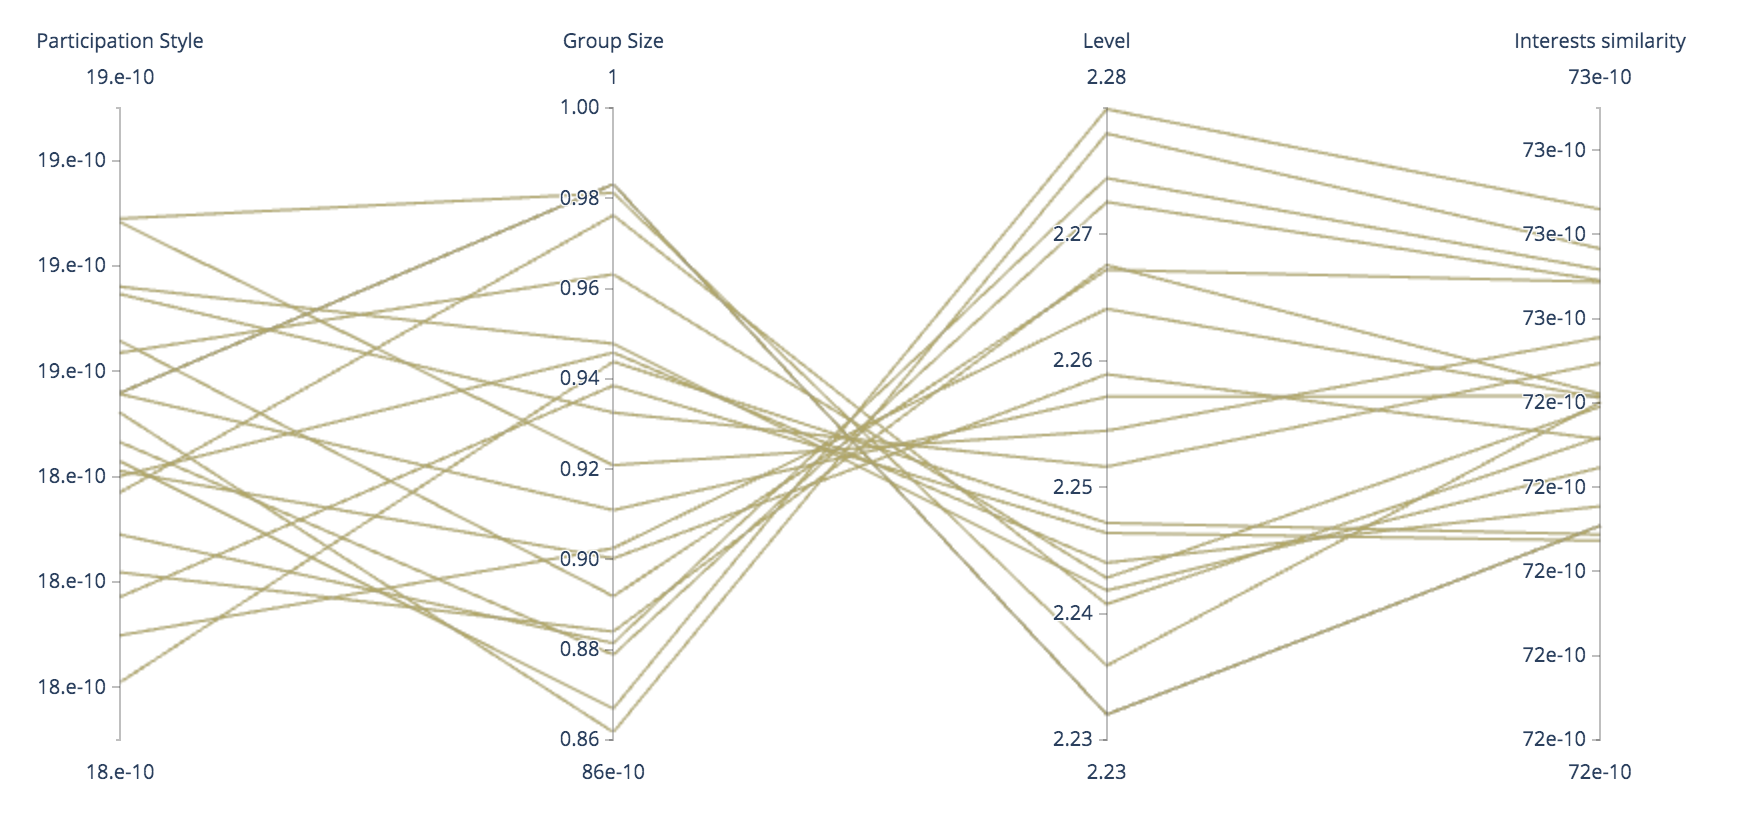
\includegraphics[width=\textwidth]{images/parallel_ref_2000.png}
    \caption{Reference front for the $n=2,000$ problem. }
    \label{fig:reference_front_2000}
\end{figure}

\subsection{Searching for Reference Parameters}
\label{sub:section_ref_params}

After some empiric testing with several values for the number of generations or steps $s$ and the population size $p$, there was a significant rise in complexity, especially for the high problem of $n=2,000$. This resulted in some experiments running for several hours and an overuse of memory space, even after using memorisation for the evaluation of costly objective functions. So, there is a bias to chose a pair small enough to maintain the complexity low, but high enough to produce a significant comparison.\\

Considering that a fair comparison requires a level of complexity similar to each algorithm, this research used the same parameters for $s$ and $p$, and the same operators for each of the algorithms. It should be noted that not all the algorithms used both of these parameters, but they were considered because they were shared across most of the algorithms.\\

In this experiment, several combinations of these parameters were tested for SOA and MOA. For the SOA, a generational GA was used, whereas, for the MOA, the algorithm NSGA-II was used. These pairs of parameters $(p,s)$ to be tested were established on a constant scale: \textbf{100}, \textbf{150}, \textbf{200}, \textbf{250}, and \textbf{300}. This experiment only considered the problem sizes of \textbf{20} and \textbf{200} students. Each pair of parameters was tested for \textbf{50} independent runs. Although a high performance may be observed from the high parameters, it should be considered that a pair with lower complexity is preferred.\\

Table~\ref{table:parameters_(SOA)_20} shows the results for the SOA of $n = 20$. The different metrics give a variety of results that leans towards high pairs, like $(250,300)$ or $(250,250)$. However, in Table~\ref{table:parameters_(SOA)_200}, it is observed that when the size of the problem grows to $n=200$, pairs of lower parameters show to have a better performance. \\

Table~\ref{table:parameters_(MOA)_20} shows the result for MOA with $n=20$. There, it can be observed a significant frequency for the pair $(100,300)$ for most metrics. The HV metric, however,  showed high performance for $(150,150)$ as the best, and $(100,100)$ as the second-best. Finally, Table~\ref{table:parameters_(MOA)_200} shows for $n=200$, where the most frequent pair is $(100,100)$.
%
Since it was established that there is a bias for lower complexity, the selected pair of parameters for the following experiments was $p=100$ and $s=100$.\\

\begin{table}[H]
\centering
\resizebox{\textwidth}{!}{
\begin{tabular}{lcccc}
\hline
    & Best $(p,s)$     & Best Value & Second Best $(p,s)$ & Second Best Value  \\
    \hline
    EP Mean and STD            & 150,250  & $8.77_{3.50}$ & 100,150 & $8.98_{3.90}$ \\
    EP Med and Inter Range     & 250,250  & $9.45_{2.90}$ & 300,150 & $9.46_{3.40}$ \\
    SPREAD Mean and STD        & 100,100  & $1.00_{0.00}$ & 150,100 & $1.00_{0.00}$ \\
    SPREAD Med and Inter Range & 100,100  & $1.00_{0.00}$ & 150,100 & $1.00_{0.00}$ \\
    GD Mean and STD            & 150,250  & $9.27_{3.90}$ & 250,250 & $9.29_{3.60}$ \\
    GD Med and Inter Range     & 250,300  & $9.84_{3.70}$ & 250,250 & $9.92_{3.60}$ \\
    IGD Mean and STD           & 150,250  & $2.25_{0.90}$ & 250,250 & $2.25_{0.83}$ \\
    IGD Med and Inter Range    & 250,300  & $2.40_{0.83}$ & 250,250 & $2.42_{0.88}$ \\
    IGD+ Mean and STD          & 150,250  & $9.80_{4.30}$ & 250,250 & $9.93_{3.9}$ \\
    IGD+ Med and Inter Range   & 250,300  & $10.07_{3.70}$ & 250,250 & $10.08_{3.9}$ \\
    \hline 
    \end{tabular}
}
\caption{The results of the parameters experiment of $n=20$ for SOA, by combinations of a population size $p$ and a number of steps or generations $s$.}
\label{table:parameters_(SOA)_20}
\end{table}

\begin{table}[H]
\centering
\resizebox{\textwidth}{!}{
    \begin{tabular}{lcccc}
    \hline
    & Best $(p,s)$ & Best Value & Second Best $(p,s)$ & Second Best Value   \\
    \hline
    EP Mean and STD            & 100,100 & $30.97_{5.60}$  & 200,150  & $30.99_{5.40}$   \\
    EP Med and Inter Range     & 200,150 & $30.94_{7.60}$  & 250,300  & $30.96_{8.00}$   \\
    SPREAD Mean and STD        & 100,100 &  $1.00_{0.00}$  & 150,100  & $1.00_{0.00}$   \\
    SPREAD Med and Inter Range & 100,100 &  $1.00_{0.00}$  & 150,100  & $1.00_{0.00}$   \\
    GD Mean and STD            & 100,100 &  $4.04_{5.80}$  & 200,150  & $40.05_{5.60}$   \\
    GD Med and Inter Range     & 200,150 & $40.02_{7.80}$  & 250,300  & $40.03_{7.90}$   \\
    IGD Mean and STD           & 100,100 &  $9.16_{1.30}$  & 200,150  & $9.18_{1.20}$   \\
    IGD Med and Inter Range    & 200,150 &  $9.12_{1.70}$  & 250,300  & $9.15_{1.70}$   \\
    IGD+ Mean and STD          & 100,100 & $40.00_{5.90}$  & 200,150  & $40.01_{5.70}$   \\
    IGD+ Med and Inter Range   & 200,150 & $30.96_{7.90}$  & 250,300  & $30.98_{8.40}$   \\
    \hline
    \end{tabular}
}
\caption{The results of the parameters experiment of $n=200$ for SOA, by combinations of a population size $p$ and a number of steps or generations $s$.}
\label{table:parameters_(SOA)_200}
\end{table}

\begin{table}[H]
\centering
\resizebox{\textwidth}{!}{%
\begin{tabular}{lcccc}
\hline
                           & Best $(p,s)$   & Best Value             & Second Best $(p,s)$ & Second Best Value  \\
\hline
EP Mean and STD            & 100,300 & $2.83_{2.2}$     & 300,100 & $3.08_{2.4}$ \\
EP Med and Inter Range     & 200,300 & $1.63_{4.3}$     & 100,300 & $1.69_{4.0}$ \\
SPREAD Mean and STD        & 100,100 & $1.00_{0.0}$     & 150,100 & $1.00_{0.0}$ \\
SPREAD Med and Inter Range & 100,100 & $1.00_{0.0}$     & 150,101 & $1.00_{0.0}$ \\
GD Mean and STD            & 100,300 & $0.14_{0.14}$    & 300,300 & $0.18_{0.18}$ \\
GD Med and Inter Range     & 100,300 & $0.08_{0.24}$    & 200,300 & $0.08_{0.29}$ \\
IGD Mean and STD           & 100,300 & $0.71_{0.54}$    & 300,100 & $0.75_{0.59}$ \\
IGD Med and Inter Range    & 100,300 & $0.41_{0.89}$    & 300,100 & $0.41_{0.98}$ \\
IGD+ Mean and STD          & 100,300 & $2.89_{2.5}$     & 300,100 & $3.19_{2.7}$ \\
IGD+ Med and Inter Range   & 200,300 & $1.48_{4.5}$     & 100,250 & $1.64_{7.1}$ \\
HV Mean and STD            & 150,150 & $0.36_{64.00}$   & 100,100 & $35.1_{59.00}$ \\
HV Med and Inter Range     & 200,100 & $9.78_{40.50}$   & 300,200 & $6.20_{34.00}$ \\
\hline
\end{tabular}
}
\caption{The results of the parameters experiment of $n=20$ for MOA, by combinations of a population size $p$ and a number of steps or generations $s$.}
\label{table:parameters_(MOA)_20}
\end{table}

\begin{table}[H]
\centering
\resizebox{\textwidth}{!}{%
\begin{tabular}{lcccc}
\hline
                           & Best $(p,s)$   & Best Value             & Second Best $(p,s)$ & Second Best Value        \\
\hline
EP Mean and STD            & 100,100 & $5.42_{2.30}$      &  100,200  & $6.37_{3.30}$ \\
EP Med and Inter Range     & 100,100 & $5.32_{2.80}$      &  100,200  & $5.64_{5.30}$ \\
SPREAD Mean and STD        & 250,300 & $1.00_{0.00}$      &  300,300  & $1.00_{0.00}$ \\
SPREAD Med and Inter Range & 150,100 & $1.00_{0.00}$      &  200,100  & $1.00_{0.00}$ \\
GD Mean and STD            & 100,200 & $0.46_{0.24}$      &  100,300  & $0.50_{0.23}$ \\
GD Med and Inter Range     & 100,200 & $0.40_{0.35}$      &  100,150  & $0.50_{0.51}$ \\
IGD Mean and STD           & 100,100 & $1.24_{0.50}$      &  100,150  & $1.50_{0.74}$ \\
IGD Med and Inter Range    & 100,100 & $1.18_{0.62}$      &  100,200  & $1.34_{1.20}$ \\
IGD+ Mean and STD          & 100,100 & $5.33_{2.30}$      &  100,150  & $6.37_{3.50}$ \\
IGD+ Med and Inter Range   & 100,100 & $5.21_{3.00}$      &  100,200  & $5.47_{5.20}$ \\
HV Mean and STD            & 300,200 & $440.00_{570.00}$  &  300,250  & $449.00_{640.00}$ \\
HV Med and Inter Range     & 300,150 & $207.00_{420.00}$  &  200,250  & $239.00_{390.00}$ \\
\hline
\end{tabular}%
}
\caption{The results of the parameters experiment of $n=200$ for MOA, by combinations of a population size $p$ and a number of steps or generations $s$.}
\label{table:parameters_(MOA)_200}
\end{table}

\section{Implementation Details}

In this section, the descriptions for all the algorithms are given with each of their specific implementations for the problem. As previously noted, all the implementations were already included in the \textbf{jMetal} and \textbf{JAMES} frameworks, and the only extra functions created were the mutation and crossover operators which were detailed in Section~\ref{3.4}.

\subsection{Single-Objective Algorithms}
\label{sub:soa_implementation}

A disadvantage found in the experiments of Chapter~\ref{chapter:chapter04} was that for the SOA, the ranges of each of the objective functions varied considerably, which added more weight for the higher evaluation results. This issue is addressed using {\em a posteriori} normalisation of the parameters, which are computed with Equation~(\ref{eq:normalization_equation}) based on the bounds given in Table~\ref{table:normalization_parameters}. \\

The full details of each of the implementations can be seen in Table~\ref{table:(SOA)_details_jmetal} for the algorithms used present in the jMetal framework.  Table~\ref{table:(SOA)_details_james} presents for the algorithms used in the James framework.

\begin{equation}
    v_{norm} = \frac{v- v_{min}}{v_{max} - v_{vmin}} 
    \label{eq:normalization_equation}
\end{equation}

\begin{table}[H]
    \begin{tabular}{lcc}
    \hline
    Objective function & Minimum value $v_{min}$ & Maximum value $v_{max}$ \\
    \hline
    Group Size Function                  & 0.50  & 1.50 \\
    Participation Style Function         & 0.00  & 1.00 \\
    Level Function                       & 0.00  & 2.82 \\
    Interests Cosine Similarity Function & 0.00  & 1.00 \\
    \hline
    \end{tabular}
    \caption{The $v_{min}$ and $v_{max}$ values for each objective function used in the normalisation.}
    \label{table:normalization_parameters}
\end{table}

\begin{table}[H]
    \begin{tabular}{p{0.15\textwidth}p{0.15\textwidth}p{0.30\textwidth}p{0.24\textwidth}p{0.10\textwidth}}
    \hline
    Denomination  & Full name & Details & Additional Parameters
    \\
    \hline
    GGA & Genetic Generational Algorithm & Is an implementation of the Genetic Algorithm in which all the solutions are replaced in each of the generations. & n/a \\ \\
    GSA & Genetic Steady Algorithm & Is an implementation of the Genetic Algorithm in which a single solution is added and another one is eliminated in each generation & n/a \\ \\
    ES & Elitist Strategy Algorithm $(\mu + \lambda)$ & Randomly selects a parent form the set of $\mu$ individuals from both the parents and offspring of the last generation, the parent is then mutated and generates $\lambda$ offsprings. & $\mu = 1$; $\lambda = pop (100)$ \\ \\
    NES & Non-Elitist Strategy Algorithm $(\mu,\lambda)$ & Randomly selects a parent form the set of $\mu$ individuals from both the parents and offspring of the last generation, and the parent is then mutated and generates $\lambda$ offsprings  & $\lambda = pop (100)$ \\ \\
    LS & Local Search (Steepest Descent/Hill Climbing) & The implementation found in the framework jMetal, was the one used as a middle step procedure for other algorithms like $ABYSS$. it makes use of a Dominance comparator & $\epsilon = 0$ \\ \\
    SORS & Random Search & n/a & n/a  \\ \\
    \hline
    \end{tabular}
    \caption{Specific details of the Single-Objective Algorithms Implementations based on the jMetal Framework.}
    \label{table:(SOA)_details_jmetal}
\end{table}

\begin{table}[H]
    \begin{tabular}{p{0.15\textwidth}p{0.15\textwidth}p{0.30\textwidth}p{0.24\textwidth}p{0.10\textwidth}}
    \hline
    Denomination  & Full name & Details & Additional Parameters 
    \\
    \hline
    RD & Random Descent & The neighbourhood is considered as a mutation step, so all the possible mutations are considered in each step. & n/a \\ \\
    PT & Parallel Tempering (Replica Exchange Monte Carlo) & Similar to Simulated Annealing this algorithm uses a max temperature and a low temperature, also running parallel replicas of Metropolis search.& $temp_{min} = 1 * 1e^{-8}$;$temp_{max} = 1 * 0.6$; $steps_{max} = 100$; $replicas = 2$ \\ \\
    \hline
    \end{tabular}
    \caption{Specific details of the Single-Objective Algorithms Implementations based on the James Framework.}
    \label{table:(SOA)_details_james}
\end{table}

\subsubsection{Multi-Objective algorithms}

The details and specific parameters for the multi-objective algorithms can be seen in Table~\ref{table:(MOA)_details}. In this case, all the algorithms implementations belong to the jMetal framework. It should also be noted that a binary tournament selection, a ranking, and crowding distance were used for all these algorithms.

\begin{table}[H]
    \begin{tabular}{p{0.15\textwidth}p{0.15\textwidth}p{0.30\textwidth}p{0.30\textwidth}}
    \hline
    Denomination  & Full Name & Details & Additional parameters \\
    \hline
    ESPEA         & Electrostatic Potential Energy Evolutionary Algorithm  & Since no scalarized preference is specified, uniform preferences are assumed
    Uses a Worst in Archive Replacement Strategy. 
    Where Among all eligible archive members that can be replaced the one exhibiting the largest energy contribution is replaced. & Replacement Strategy: Worst in Archive \\ \\
    MOMBI-II        & Many Objective Metaheuristic Based on the R2 Indicator & Requires a number of weights equal to the population size. These weights were selected according to the population size using the Simplex-Lattice Design method & Vector of weights, using Simple-Lattice Design method; According to the population size. \\ \\
    NSGA-II       & Non-dominated Sorting Genetic Algorithm               & n/a & n/a \\ \\
    MORS          & Multi-Objective Random Search                                          & n/a  & n/a \\ \\ 
    SPEA-II        & Strength Pareto Evolutionary Algorithm                 & n/a  & n/a \\ \\
    \hline                                                                                                                 
    \end{tabular}
    \caption{Specific details of the Multi-Objective Algorithms Implementations.}
    \label{table:(MOA)_details}
\end{table}

\section{Scalarization Methods}
\label{sec:scalarization}

Multi-objective optimisation problems are classically solved using scalarization techniques \cite{Emmerich2018}. Scalarization means that the objective functions will be aggregated or reformed as constraints, therefore a single-objecttive problem is solved. For this research, we make use of three different scalarization methods: weighted sum, Chebyshev scalarization and $\epsilon$-constraint method which are described in this section.

\subsection{Weighted Sum Method}

Weighted sum (WS) also known as linear weighting is one of the most common ways to scalarize a multi-objective problem \cite{CooperWilliamW.2010}. Each objective function is 


\subsection{Chebyshev Scalarization}

\subsection{$\epsilon$-constraints Scalarization}

%   |  |  |/~~\|~~\ /~|~|\  |/~~\  |~~\ /\ |\  |\  |~~|~~\
%  |  |  |    |__/(  | | \ |  __  |--</__\| \ | \ |--|__/
%  \/ \/ \__/|  \ \_|_|  \|\__/  |__/    \  \|  \|__|  \

\section{Experimental Phases}
\label{sec:first_phase}

In this section, we explore the performance of the different proposed algorithms for minimising the defined objective functions described in Section~\ref{section:objective_functions}. Specially the differences of performance among SOA and MOA. Each SOA was run using different scalarization methods: WS, CHE and E-Constraints described in Section~\ref{sec:scalarization}. \\

The experiments are divided in two phases. The main difference between these experiments is the parameters for the mutation rate and the crossover rate. The first phase make use of Typical parameters, these are parameters usually found in the literature, which states a crossover probability between $0.5$ and $1.0$ and a mutation probability between $0.001$ and $0.05$ \cite{Lin2003}. Specifically for our experiments we use a crossover probability of $0.9$ and a mutation probability of $1/n$ where $n$ is the size of the problem which corresponds to the number of students. The second phase implements a more aggressive mutation based on the parameters for solving SMP found in the literature \cite{bello2016genetic}. The problem sizes considered were $20$, $200$ and $2,000$.\\

The Stopping condition for all of the algorithms is determined by the number of maximum evaluations which is determined as $Evaluations_{max} = p * s$, where $p$ is the size of the population and $s$ is the number of steps, both defined in Section~\ref{sub:section_ref_params}.\\

The SOA used were the implementations found in jMetal 5.4 for the GGA, GSA, ES, NES, LS and RS algorithms and RD and PT found in the JAMES 3.4.0 framework, as established in Tables~\ref{table:(SOA)_details_jmetal}, \ref{table:(SOA)_details_james}. The MOA used were the implementations of ESPEA, MOMBI-II, NSGA-II, MORS and SPEA-II found in the same jMetal framework, defined in Table~\ref{table:(MOA)_details}. The executions were done over a GNU/Linux machine with an Intel i7-4790 3.60GHz processor and 16Gb of RAM.\\

To evaluate the performance we made an analysis using the EPSILON, SPREAD, IGD+ and HV metrics. For the analysis we made use of a Median and Interquartile analysis in order to view which problem sizes may benefit a certain algorithm and a Friedman test is also conducted to determine the best algorithm overall according to each metric. Several graphs are also shown to check the consistency of the results. We performed 30 independent runs for all the problem sizes.\\

\subsection{Scalarization Weights}

The EPS scalarization method make use of a boundary to determine its constraints. This boundary was established using all the SOA and optimising each objective function independently for each of the problem sizes, taking the best result for each objective function and for each problem size. The results are shown in Table~\ref{tab:best_independant_results}. These were used as the boundaries for the constraints, in each step a single objective function is evaluated and the rest are used as constraints. If a function evaluation is higher than the best values it is consider that it had violated the constraint to a certain degree depending on how much higher it was.\\

% Please add the following required packages to your document preamble:
% \usepackage{graphicx}
\begin{table}[!htp]
\centering
\begin{tabular}{lcccc}
\hline
n     & Gs   & Ps   & Lvl  & Int  \\ \hline
20    & 0.50 & 0.02 & 0.67 & 0.55 \\
200   & 0.68 & 0.02 & 0.67 & 0.63 \\
2,000 & 0.86 & 0.02 & 0.69 & 0.65 \\ \hline
\end{tabular}%
\caption{The boundaries for each problem size and each function based on the best found results}
\label{tab:best_independant_results}
\end{table}

For the WS and CHE methods there was a need to define a weight for each function, and ideally the sum of them should equal to one. The weights to be used can also make easier to find the Pareto front by dragging the solutions towards its shape \cite{Emmerich2018}. For this reason, we make use of the previous best found values in Table~\ref{tab:best_independant_results} normalised, so they add up to one. The normalisation used was the following:\\

\begin{equation}
    w_i = \frac{f_i(x)}{\sum f(x)}
\end{equation}

Where $w_i$ is the weight to be used for each function, $f_i(x)$ is the best result found for this function evaluated individually and $\sum f(x)$ is the sum of all the results for each problem size. The weights are shown in Table~\ref{tab:weights_to_be_used}.\\

% Please add the following required packages to your document preamble:
% \usepackage{booktabs}
% \usepackage{graphicx}
\begin{table}[!htc]
\centering
\begin{tabular}{@{}lcccc@{}}
\toprule
n     & Gs    & Ps    & Lvl   & Int   \\ \midrule
20    & 0.285 & 0.012 & 0.385 & 0.317 \\
200   & 0.339 & 0.011 & 0.333 & 0.316 \\
2,000 & 0.386 & 0.011 & 0.311 & 0.292 \\ \bottomrule
\end{tabular}%
\caption{}
\label{tab:weights_to_be_used}
\end{table}

Interestingly, these weights are close from each other from their problem sizes. This could mean that there can be global weights to be used for any problem size. But for this research each problem size uses a different set of weights.\\

\subsection{First phase: Thumb Parameters}
\label{sec:first-phase}

The common parameters for the mutation and crossover probabilities specify to have a low mutation probability usually between $0.001$ and $0.05$ and a high crossover probability between $0.5$ and $1.0$  \cite{Lin2003}. In this research, we call these parameters "Thumb-Parameters", as they are rules of thumb to follow. For this experimentation phase, we used a crossover probability of $0.9$ and a mutation probability of $1/n$ where $n$ is the size of the problem which corresponds to the number of students. \\

Table~\ref{tab:igd+_thumb} shows the median and interquartile ranges for the IGD+ metric for all the problem sizes, for each SOA and their scalarization methods and each of the MOA. The results in dark grey are considered the best, and the ones in dark grey are the second best. The MOA show an advantage against the SOA for all the problem sizes, although they came very near especially with the CHE method. Although the performance varies for each of the problem sizes, there is a clear advantage for using the CHE and EPS methods for the SOA, using Thumb-Parameters. GSA and GGA show a very poor performance using the WS method overall. MOA results show an advantage for MORS and MOMBI-II, although the results are too close with each other, except for the $n = 200$ problem.\\

Table~\ref{tab:ep_thumb} shows the median and interquartile ranges for the EP metric. These results are consistent with the ones found with the IGD+ for the most part. Except for the second-best algorithm which goes to SPEA-II instead of MOMBI-II for the $n = 20$ problem, although the performance for these two is very similar, so this inconsistency may not be relevant.\\

\begin{table}[!htc]
\resizebox{\textwidth}{!}{%
\begin{tabular}{@{}lccccccccc@{}}
\toprule
         & \multicolumn{3}{c}{n = 20}                          & \multicolumn{3}{c}{n = 200}                          & \multicolumn{3}{c}{n = 2,0000}                      \\ \midrule
         & WS                & CHE            & EPS        & WS                & CHE            & EPS         & WS               & CHE            & EPS         \\ \midrule
GGA      & $22.77_{9.82}$    & $5.18_{2.42}$  & $6.21_{3.19}$  & $75.90_{83.62}$   & $14.45_{3.95}$ & $28.27_{10.41}$ & $27.08_{12.56}$  & $7.32_{0.59}$  & $8.80_{4.31}$   \\
GSA      & $25.46_{13.54}$   & $5.98_{1.74}$  & $8.49_{2.10}$  & $110.45_{136.11}$ & $15.31_{4.12}$ & $26.00_{9.67}$  & $43.36_{19.81}$  & $7.24_{0.39}$  & $10.04_{1.77}$  \\
ES       & $22.62_{14.96}$   & $5.12_{3.38}$  & $8.95_{2.73}$  & $55.90_{27.27}$   & $16.14_{3.08}$ & $20.64_{6.92}$  & $7.97_{0.89}$    & $7.56_{0.62}$  & $7.62_{0.74}$   \\
NES      & $25.49_{10.84}$   & $5.29_{3.47}$  & $8.36_{2.38}$  & $61.79_{63.46}$   & $15.74_{2.79}$ & $20.04_{4.73}$  & $8.24_{1.46}$    & $7.54_{0.73}$  & $7.59_{0.77}$   \\
LS       & $12.94_{7.16}$    & $6.73_{1.95}$  & $6.40_{1.72}$  & $15.66_{5.67}$    & $17.08_{4.59}$ & $16.81_{4.51}$  & $7.60_{0.55}$    & $7.51_{0.67}$  & $7.51_{0.77}$   \\
RD       & $10.66_{5.50}$    & $6.32_{1.92}$  & $5.73_{1.95}$  & $18.19_{2.59}$    & $16.97_{5.39}$ & $15.84_{5.05}$  & $7.40_{0.49}$    & $7.51_{0.65}$  & $7.58_{0.63}$   \\
PT       & $22.48_{10.26}$   & $4.33_{2.40}$  & $4.73_{2.13}$  & $30.65_{15.33}$   & $15.52_{3.80}$ & $21.24_{8.34}$  & $7.76_{0.58}$    & $7.51_{0.64}$  & $7.50_{0.73}$   \\
SORS     & $12.60_{5.61}$    & $6.43_{2.93}$  & $5.81_{1.82}$  & $17.43_{4.24}$    & $13.39_{1.77}$ & $18.22_{6.02}$  & $7.84_{0.93}$    & $7.19_{0.71}$  & $7.69_{0.57}$   \\ \midrule
ESPEA    & \multicolumn{3}{c}{$3.17_{1.10}$}                   & \multicolumn{3}{c}{$13.51_{3.75}$}                   & \multicolumn{3}{c}{\cellcolor{gray25}$6.28_{0.36}$} \\
MOMBI-II & \multicolumn{3}{c}{\cellcolor{gray25}$2.81_{1.46}$} & \multicolumn{3}{c}{\cellcolor{gray95}$6.03_{6.81}$}  & \multicolumn{3}{c}{$6.91_{0.40}$}                   \\
NSGA-II  & \multicolumn{3}{c}{$3.02_{1.48}$}                   & \multicolumn{3}{c}{$13.13_{1.79}$}                   & \multicolumn{3}{c}{$6.41_{0.27}$}                   \\
SPEA-II  & \multicolumn{3}{c}{$2.82_{1.43}$}                   & \multicolumn{3}{c}{$11.93_{4.19}$}                   & \multicolumn{3}{c}{$6.32_{0.42}$}                   \\
MORS     & \multicolumn{3}{c}{\cellcolor{gray95}$2.25_{1.28}$} & \multicolumn{3}{c}{\cellcolor{gray25}$6.89_{1.15}$}  & \multicolumn{3}{c}{\cellcolor{gray95}$5.67_{0.05}$} \\ \bottomrule
\end{tabular}%
}
\caption{Median and Interquartile Range for the IGD+. Metric using Thumb-Parameters}
\label{tab:igd+_thumb}
\end{table}


% Please add the following required packages to your document preamble:
% \usepackage{booktabs}
% \usepackage{graphicx}
\begin{table}[!htc]
\resizebox{\textwidth}{!}{%
\begin{tabular}{@{}lccccccccc@{}}
\toprule
         & \multicolumn{3}{c}{n = 20}                          & \multicolumn{3}{c}{n = 200}                          & \multicolumn{3}{c}{n = 2,0000}                      \\ \midrule
         & WS                & CHE            & Epsilon        & WS                & CHE            & Epsilon         & WS               & CHE            & Epsilon         \\ \midrule
GGA      & $20.15_{10.89}$   & $4.66_{1.81}$  & $6.38_{3.11}$  & $75.72_{84.29}$   & $14.96_{3.95}$ & $28.50_{10.41}$ & $26.48_{12.93}$  & $7.85_{0.59}$  & $9.32_{3.81}$   \\
GSA      & $23.10_{13.79}$   & $5.10_{1.27}$  & $8.80_{2.04}$  & $109.84_{136.94}$ & $15.84_{4.11}$ & $26.22_{9.80}$  & $42.41_{20.35}$  & $7.77_{0.39}$  & $10.42_{1.68}$  \\
ES       & $21.57_{15.65}$   & $4.72_{2.00}$  & $9.25_{2.73}$  & $56.00_{27.38}$   & $16.66_{3.07}$ & $21.10_{6.94}$  & $8.49_{0.87}$    & $8.08_{0.60}$  & $8.14_{0.74}$   \\
NES      & $24.45_{9.80}$    & $4.48_{2.20}$  & $8.49_{2.56}$  & $62.02_{63.56}$   & $16.28_{2.79}$ & $20.45_{4.63}$  & $8.75_{1.43}$    & $8.07_{0.74}$  & $8.11_{0.75}$   \\
LS       & $12.77_{8.08}$    & $6.03_{2.58}$  & $5.76_{1.33}$  & $16.18_{5.69}$    & $17.59_{4.58}$ & $17.30_{4.61}$  & $8.11_{0.54}$    & $8.02_{0.67}$  & $8.04_{0.76}$   \\
RD       & $10.12_{6.84}$    & $5.88_{1.74}$  & $5.14_{1.77}$  & $18.65_{2.64}$    & $17.46_{5.39}$ & $16.25_{5.13}$  & $7.91_{0.50}$    & $8.03_{0.66}$  & $8.10_{0.62}$   \\
PT       & $22.33_{10.77}$   & $4.00_{2.06}$  & $5.07_{2.42}$  & $30.82_{15.47}$   & $16.05_{3.80}$ & $21.53_{8.04}$  & $8.26_{0.58}$    & $8.04_{0.63}$  & $8.02_{0.74}$   \\
SORS     & $12.08_{6.81}$    & $5.64_{2.43}$  & $5.18_{1.27}$  & $17.87_{4.27}$    & $13.93_{1.77}$ & $18.72_{5.99}$  & $8.31_{0.95}$    & $7.72_{0.71}$  & $8.20_{0.57}$   \\ \midrule
ESPEA    & \multicolumn{3}{c}{$3.49_{1.23}$}                   & \multicolumn{3}{c}{$14.00_{3.77}$}                   & \multicolumn{3}{c}{\cellcolor{gray25}$6.81_{0.37}$} \\
MOMBI-II & \multicolumn{3}{c}{$3.09_{1.15}$}                   & \multicolumn{3}{c}{\cellcolor{gray95}$6.57_{7.02}$}  & \multicolumn{3}{c}{$7.44_{0.40}$}                   \\
NSGA-II  & \multicolumn{3}{c}{$3.12_{1.25}$}                   & \multicolumn{3}{c}{$13.55_{1.70}$}                   & \multicolumn{3}{c}{$6.93_{0.26}$}                   \\
SPEA-II  & \multicolumn{3}{c}{\cellcolor{gray25}$2.82_{1.27}$} & \multicolumn{3}{c}{$12.26_{4.10}$}                   & \multicolumn{3}{c}{$6.84_{0.41}$}                   \\
MORS     & \multicolumn{3}{c}{\cellcolor{gray95}$2.54_{0.91}$} & \multicolumn{3}{c}{\cellcolor{gray25}$7.39_{1.19}$}  & \multicolumn{3}{c}{\cellcolor{gray95}$6.19_{0.04}$} \\ \bottomrule
\end{tabular}%
}
\caption{Median and Interquartile Range for the EP. Metric using Thumb-Parameters}
\label{tab:ep_thumb}
\end{table}

Tables~\ref{tab:spread_thumb} and \ref{tab:hv_thumb} show the results for the SPREAD and HV metrics respectively. These are only evaluated for the MOA since the SOA only has a single point in the front per run, therefore for them the spread would always be one. The HV is calculated using the inverse of the front, so a higher HV is considered better.\\ 

The two best algorithms according to the HV metric are NSGA-II and SPEA-II. These results are mostly consist ant between problem sizes. These results are mostly consistent with the SPREAD showed in Table~\ref{tab:spread_thumb}. EP and IGD+ highlighted MORS as the better algorithm, but as previously noted, the difference between the others in comparison wasn't much. Therefore the analysis of HV showed clearer results among the MOA. While EP and IGD+ showed an slight advantage for the MOA against the SOA in general.\\
  
% Please add the following required packages to your document preamble:
% \usepackage{booktabs}
% \usepackage{graphicx}
\begin{table}[!htc]
\centering
\begin{tabular}{@{}lccc@{}}
\toprule
         & n = 20                          & n = 200                         & n = 2,000         \\ \midrule
ESPEA    & $0.65_{0.09}$                   & $1.00_{0.31}$                   & $1.05_{0.05}$                   \\
MOMBI-II & $0.78_{0.06}$                   & $0.88_{0.06}$                   & $1.00_{0.01}$                   \\
NSGA-II  & \cellcolor{gray95}$0.56_{0.06}$ & \cellcolor{gray95}$0.81_{0.18}$ & $0.91_{0.07}$                   \\
SPEA-II  & \cellcolor{gray25}$0.60_{0.08}$ & \cellcolor{gray25}$0.82_{0.09}$ & \cellcolor{gray95}$0.84_{0.06}$ \\
MORS     & $0.68_{0.11}$                   & $0.83_{0.04}$                   & \cellcolor{gray25}$0.88_{0.02}$ \\ \bottomrule
\end{tabular}%
\caption{Median and Interquartile Range for the SPREAD Metric using Thumb-Parameters}
\label{tab:spread_thumb}
\end{table}

% Please add the following required packages to your document preamble:
% \usepackage{booktabs}
% \usepackage{graphicx}
\begin{table}[!htc]
\centering
\begin{tabular}{@{}lccc@{}}
\toprule
         & n = 20                                    & n = 200                                   & n = 2,000                                 \\ \midrule
ESPEA    & $  8.00e+02_{ 6.3e+02}$                   & $  3.83e+05_{ 1.3e+06}$                   & $  1.68e+05_{ 1.5e+05}$                   \\
MOMBI-II & $  1.59e+02_{ 1.5e+02}$                   & $  3.29e+04_{ 5.2e+04}$                   & $  1.72e+03_{ 3.9e+02}$                   \\
NSGA-II  & \cellcolor{gray95}$  1.25e+03_{ 1.2e+03}$ & \cellcolor{gray95}$  1.13e+06_{ 2.2e+06}$ & \cellcolor{gray25}$  6.93e+05_{ 5.0e+05}$ \\
SPEA-II  & \cellcolor{gray25}$  9.85e+02_{ 1.3e+03}$ & \cellcolor{gray25}$  4.45e+05_{ 1.1e+06}$ & \cellcolor{gray95}$  1.04e+06_{ 7.0e+05}$ \\
MORS     & $  1.61e+02_{ 4.2e+02}$                   & $  1.37e+05_{ 7.9e+04}$                   & $  2.57e+04_{ 1.2e+04}$                   \\ \bottomrule
\end{tabular}%
\caption{Median and Interquartile Range for the HV. Metric using Thumb-Parameters}
\label{tab:hv_thumb}
\end{table}

A Friedman ranking test was done to define which algorithms performed better across all problem sizes. The results for the ranking test on the IGD+ and EP metrics are shown in Tables~\ref{tab:fried_igd+_thumb} and \ref{tab:fried_ep_thumb}. The ranking for both of them are pretty close to each other for SOA and for the MOA is exactly the same. There is a clear advantage for using the CHE method with the SOA. There is not a clear best SOA as PT and GSA can considered the best according to each of the rankings, although they remain very close to SORS and GGA. \\ 

Both rankings show an overall better performance for the MOA, although, these metrics are not able to determine a best algorithm among themselves, since their position in the ranking is very close.\\

\begin{table}[!htc]
\centering
\begin{tabular}{lc}
\toprule
Algorithm  & Ranking \\
\midrule
GGA_{WS}   & 27.66  \\
GSA_{WS}   & 28.66  \\
ES_{WS}    & 25.33  \\
NES_{WS}   & 27.00  \\
LS_{WS}    & 19.00  \\
RD_{WS}    & 16.00  \\
PT_{WS}    & 23.66  \\
SORS_{WS}  & 21.00  \\
\midrule
GGA_{CHE}  & 9.00   \\
GSA_{CHE}  & 8.66   \\
ES_{CHE}   & 12.33  \\
NES_{CHE}  & 11.66  \\
LS_{CHE}   & 14.00  \\
RD_{CHE}   & 15.66  \\
PT_{CHE}   & 8.00   \\
SORS_{CHE} & 8.66   \\
\midrule
GGA_{EPS}  & 22.00  \\
GSA_{EPS}  & 23.33  \\
ES_{EPS}   & 20.66  \\
NES_{EPS}  & 17.66  \\
LS_{EPS}   & 14.33  \\
RD_{EPS}   & 12.66  \\
PT_{EPS}   & 16.00  \\
SORS_{EPS} & 17.00  \\
\midrule
ESPEA      & 3.66   \\
MOMBI-II   & 3.66   \\
NSGA-II    & 3.66   \\
SPEA-II    & 2.66   \\
MORS       & 1.33   \\
\bottomrule
\end{tabular}
\caption{Friedman Ranking on IGD+ metric using Thumb-Parameters}
\label{tab:fried_igd+_thumb}
Considering reduction performance (distributed according to chi-square with 28 degrees of freedom: 74.63).
\end{table}

\begin{table}[!htp]
\centering
\begin{tabular}{lc}
\toprule
Algorithm&Ranking\\
\midrule
GGA_{WS}&27.00\\
GSA_{WS}&29.00\\
ES_{WS}&25.66\\
NES_{WS}&26.66\\
LS_{WS}&19.00\\
RD_{WS}&16.33\\
PT_{WS}&23.99\\
SORS_{WS}&20.66\\
\midrule
GGA_{CHE}&8.33\\
GSA_{CHE}&7.66\\
ES_{CHE}&12.66\\
NES_{CHE}&11.66\\
LS_{CHE}&13.66\\
RD_{CHE}&15.33\\
PT_{CHE}&8.00\\
SORS_{CHE}&8.66\\
\midrule
GGA_{EPS}&23.00\\
GSA_{EPS}&23.33\\
ES_{EPS}&20.66\\
NES_{EPS}&17.66\\
LS_{EPS}&14.00\\
RD_{EPS}&12.33\\
PT_{EPS}&17.66\\
SORS_{EPS}&17.00\\
\midrule
ESPEA&3.66\\
MOMBI-II&3.66\\
NSGA-II&3.66\\
SPEA-II&2.66\\
MORS&1.33\\
\bottomrule
\end{tabular}
\caption{Friedman Ranking on EP. metric using Thumb-Parameters}
\label{tab:fried_ep_thumb}
Considering reduction performance (distributed according to chi-square with 28 degrees of freedom: 76.24).
\end{table}


The rankings for SPREAD and HV metrics are shown in Tables~\ref{tab:fried_spread_thumb} and \ref{tab:hv_thumb} respectively. For the Friedman test on the HV metric the higher is the better result. The best algorithms according to this ranking are SPEA-II and NSGA-II separated only by a small difference. SPEA-II shows a lower SPREAD metric which means their solutions are more convergent.\\
 
\begin{table}[!htc]
\centering
\begin{tabular}{lc}
\toprule
Algorithm&Ranking\\
\midrule
ESPEA&4.33\\
MOMBI-II&3.66\\
NSGA-II&2.66\\
SPEA-II&1.99\\
MORS&2.33\\
\bottomrule
\end{tabular}
\caption{Friedman Ranking on SPREAD metric using Thumb Parameters}
\label{tab:fried_spread_thumb}
Considering reduction performance (distributed according to chi-square with 4 degrees of freedom: 4.53).
\end{table}

\begin{table}[!htc]
\centering
\begin{tabular}{lc}
\toprule
Algorithm&Ranking\\
\midrule
ESPEA&3.33\\
MOMBI-II&1.00\\
NSGA-II&4.66\\
SPEA-II&4.00\\
MORS&2.00\\
\bottomrule
\end{tabular}
\caption{Friedman Ranking on HV metric using Thumb Parameters}
\label{tab:fried_hv_thumb}
\end{table}

% Once the performance of both approaches in terms of the Pareto front approximation is almost the same, we present the comparison in terms of the classification performance of the full models selected for each method.

In this section we tested both SOA and MOA using Thumb-Parameters, which involve the mutation rate and the crossover among the different algorithms.

\subsection{Second Phase}
\label{sec:second-phase}

%---

\subsection{Stability evaluation}

To test the stability, an experiment took place measuring the results from the previous set of exploratory experiments for the $n=20$ problem. The results were evaluated using the methodology described in Section~\ref{section:stability}. The number of stable students is considered for each preference criteria. And by each of the tested algorithms. The analysis was made using a metaheuristic LS, the single objective genetic algorithm GGA and the multi-objective algorithm NSGA-II. Using a random solution for comparison.\\

Results are shown in Table~\ref{tab:preference_criteria}, here the solutions obtained from the algorithms are compared to a random solution, it can be seen that the stability improves or stays the same for all the algorithms, except for the $Lvl$ criteria. This can be explained because of the little variation between the levels of the students. Interestingly, NSGA-II seems to have the most stability spread across all the objective functions.\\

% Please add the following required packages to your document preamble:
% \usepackage{graphicx}
\begin{table}[H]
\centering
\resizebox{\textwidth}{!}{%
\begin{tabular}{lcccc}
\hline
 & $Gs-Stable$ & $Ps-Stable$ & $Int-Stable$ & $Lvl-Stable$ \\
 \hline
Random Solution & 3 & 0 & 0 & 12 \\
Local Search & 6 & 3 & 0 & 7 \\
Genetic Generational Algorithm & 8 & 0 & 2 & 7 \\
NSGA-II & 3 & 2 & 2 & 9 \\
\hline
\end{tabular}%
}
\caption{Number of stable students in the groups by preference criteria}
\label{tab:preference_criteria}
\end{table}

This analysis was made not to test which algorithm lead to the most stability, but to ensure that by optimising the objective functions it can lead to higher stability. However, in future research, it might be possible to have a deeper analysis of the behaviour of the stability of this problem.
    
\section{Correlation between the results}

After extensive analysis and looking at the results and observing an apparent trade-off between some of the objective functions There was the need of analysing the correlation among objectives over the non-dominated, which were taken from the best front obtained from the $n=200$ problem.\\

For this correlation analysis, a Pearson's Correlation test was used taking into account all the objective functions results and their correlation between each other.

% Please add the following required packages to your document preamble:
% \usepackage{graphicx}
\begin{table}[H]
\centering

\begin{tabular}{lll}
\hline
Objective Functions & Statistic & P-value \\
\hline
Group Size and Participation Style & $0.50$ & $2.17e-08$ \\
Group Size and Level & $-0.96$ & $2.04e-17$ \\
Group Size and Interests Similarity & $-0.57$ & $4.57e-11$ \\
Participation Style and Level & $-0.55$ & $3.26e-10$ \\
Participation Style and Interests Similarity & $0.03$ & $0.74$ \\
Level and Interests Similarity & $0.69$ & $2.04e-17$ \\
\hline
\end{tabular}%

\caption{Results of the Pearson correlation analysis}
\label{tab:correlation}
\end{table}

Taking the results from Table~\ref{tab:correlation}, The null Hypothesis of being two independent sets is rejected in all the comparisons except for the $Ps$ and the $Int$ functions using a less than one per cent significance. This means All the objective functions are correlated except for these two. However, for the $Gs$ in respect to the $Lvl$ and $Int$, there seems to be a negative correlation, the same with the $Ps$ and $Lvl$. This was also observed visually in Figure~\ref{fig:parallel_2000} and others, where SOA seem to achieve better results for the $Lvl$ and MOA better results for the $Ps$ function.\\

It also makes sense for the $Gs$  to be correlated to the $Ps$ since the more members are in a group since the more people are in the group, the more participation will take place in the group. $Gs$ and $Lvl$ are negatively correlated, which also makes sense, since the higher the members of the group.
This also validates more the use of MOA over SOA, since there are at least two objective functions which are not correlated.